\documentclass{article}

\usepackage{arxiv}

\usepackage[utf8]{inputenc} % allow utf-8 input
\usepackage[T1]{fontenc}    % use 8-bit T1 fonts
\usepackage[hidelinks]{hyperref}       % hyperlinks
\usepackage{url}            % simple URL typesetting
\usepackage{booktabs}       % professional-quality tables
\usepackage{amsmath,amssymb,amsthm}
\usepackage{amsfonts}       % blackboard math symbols
\usepackage{nicefrac}       % compact symbols for 1/2, etc.
\usepackage{microtype}      % microtypography
\usepackage{mathrsfs}
\usepackage{graphicx}
\usepackage{doi}
\usepackage{acronym}
\usepackage{listings}
\usepackage{tikz}
\usepackage[backend=biber,style=ieee]{biblatex}

\addbibresource{references.bib}

\usetikzlibrary{trees}

\newacro{abm}[ABM]{Agent-Based Model}
\newacro{cabm}[CABM]{Cellular Agent-Based Model}
\newacro{ca}[CA]{Cellular Automaton}
\newacroplural{ca}[CA]{Cellular Automata}

\title{Rust for Scientific Computing}

%\date{September 9, 1985}	% Here you can change the date presented in the paper title
%\date{} 					% Or removing it

\author{
    \href{https://orcid.org/0009-0001-0613-7978}{
        
\includegraphics[scale=0.06]{orcid.pdf}
        \hspace{1mm}Jonas Pleyer
    }
    \thanks{
        \href{https://jonas.pleyer.org}{jonas.pleyer.org},
        \href{https://cellular-raza.com}{cellular-raza.com}
    }\\
	Freiburg Center for Data-Analysis and Modeling\\
	University of Freiburg\\
	\texttt{jonas.pleyer@fdm.uni-freiburg.de} \\
	%% examples of more authors
	\And
	\href{https://orcid.org/0000-0002-6371-4495}{
        
\includegraphics[scale=0.06]{orcid.pdf}
        \hspace{1mm}Christian Fleck
    }\\
	Freiburg Center for Data-Analysis and Modeling\\
	University of Freiburg
}

% Uncomment to remove the date
%\date{}

% Uncomment to override  the `A preprint' in the header
\renewcommand{\headeright}{Preprint}
%\renewcommand{\undertitle}{Technical Report}
\renewcommand{\shorttitle}{Rust for High-Performance Computing}

\usepackage{enumitem}
\setlist{nolistsep}

%%% Add PDF metadata to help others organize their library
%%% Once the PDF is generated, you can check the metadata with
%%% $ pdfinfo template.pdf
\hypersetup{
pdftitle={Rust for High-Performance Computing},
pdfsubject={q-bio.NC, q-bio.QM},
pdfauthor={Jonas Pleyer, Christian Fleck},
pdfkeywords={},
}

% Change numbering of equations
% \numberwithin{equation}{section}

% MAKE TITLES IN THEOREMS BOLD
\makeatletter
\def\th@plain{%
  \thm@notefont{}% same as heading font
  \itshape % body font
}
\def\th@definition{%
  \thm@notefont{}% same as heading font
  \normalfont % body font
}
\makeatother

\begin{document}
\maketitle

%###################################################################################################
\begin{abstract}
\end{abstract}

\pagebreak
\tableofcontents
\pagebreak

% keywords can be removed
\keywords{Rust \and HPC \and High-Performance Computing \and Programming}

%###################################################################################################
\section{Introduction}
\label{section:introduction}

General Remarks about languages
\begin{enumerate}
    \item Programming languages allow us to express machine instructions in human-readable code.
    \item Depend on use-case
    \item Translate human-interpretable code into machine instructions
    \item tradeoff between high-level view (abstraction) and performance (low level)
    \item C++ has "zero-cost" abstractions
\end{enumerate}

Importance of programming in science
\begin{enumerate}
    \item New fields of study (computational physics, chemistry, biology, sociology, etc.)
    \item Cite some groundbreaking examples which were possible due to programming in science (maybe
          weather)
    \item
\end{enumerate}

Judging C/C++
\begin{enumerate}
    \item Previous Decades: C/C++ in science
    \item Limitations of design choices of language become evident
    \item fragmented ecosystem; good for competition; bad for developer experience
    \item modern features missing: package manager with package registries, build system
    \item technical details; mutable by default, templates vs generics, backwards compatiblity
          becomes a problem ("there is a much simpler langauge within C++ that tries to get out"),
          macros, no clear ownership rules on a language level, dangling pointers
    \item still many good principles (such as RAII) and design principles/concepts (cite gang of
          four)
\end{enumerate}

The need for modern languages
\begin{enumerate}
    \item Java aimed to replace C due to pointers
    \item Go also aims to replace it, go is garbage-collected; thus cannot be as well-performing as
          C++ or C
    \item Python, Javascript for high-level abstractions ("as glue"); no performance howerver
\end{enumerate}

Elaborate on why Rust solves many problems
\begin{enumerate}
    \item safety guarantees; ensures that code which we write actually performs what we set out to
          do
    \item no dangling pointers
    \item zero-cost abstrations
    \item compiled without garbage-collector
    \item tooling: modern ecosystem; package manager, build system, package registry
    \item strong type system which is generally considered sound
    \item macro system gets type-checked
    \item very good C-interop; utilize existing software
\end{enumerate}

Show that many companies are starting to adopt Rust
\begin{enumerate}
    \item Amazon (AWS)\\
          AWS developed Firecracker, a microVM monitoring service powering AWS Lambda and AWS
          Fargate.
          Firecracker is built primarily in Rust to offer fast cold boot times and secure
          workload isolation.
    \item Rust-supported runtimes like AWS Lambda also allow developers to write serverless
          functions using Rust.
    \item Google\\
          Fuchsia, Google's modern operating system, uses Rust extensively for system components
          such as drivers and services to enhance security and reliability.
    \item Google (Android)\\
          Android integration: Rust has been adopted within the Android Open Source Project (AOSP)
          to improve memory safety in critical system components. DEV Community Litslink
    \item Meta (Facebook)\\
          Mononoke, Facebook’s large-scale source control backend for Mercurial, was written in
          Rust to improve performance and reliability in its monorepo.
    \item Meta (Facebook)\\
          Facebook employs Rust in developing CLI tools, distributed systems, and cron jobs.
          Engineers write millions of lines of Rust internally.
    \item Apple\\
          Apple’s Cloud Traffic team and backend infrastructure have been shifting from C to Rust,
          with new functionality being primarily built in Rust. This change was driven by
          performance, security, and developer efficiency goals. Reddit
    \item Microsoft\\
          Although not part of FAANG, it’s noteworthy—Microsoft is rewriting parts of the Windows
          kernel and system components in Rust (e.g., DWriteCore, GDI Regions), prioritizing memory
          safety.
    \item Azure services-like Azure IoT Edge—also incorporate Rust.
    \item Linux Kernel\\
          Only other supported language except from C
\end{enumerate}

\begin{figure}
    \centering
    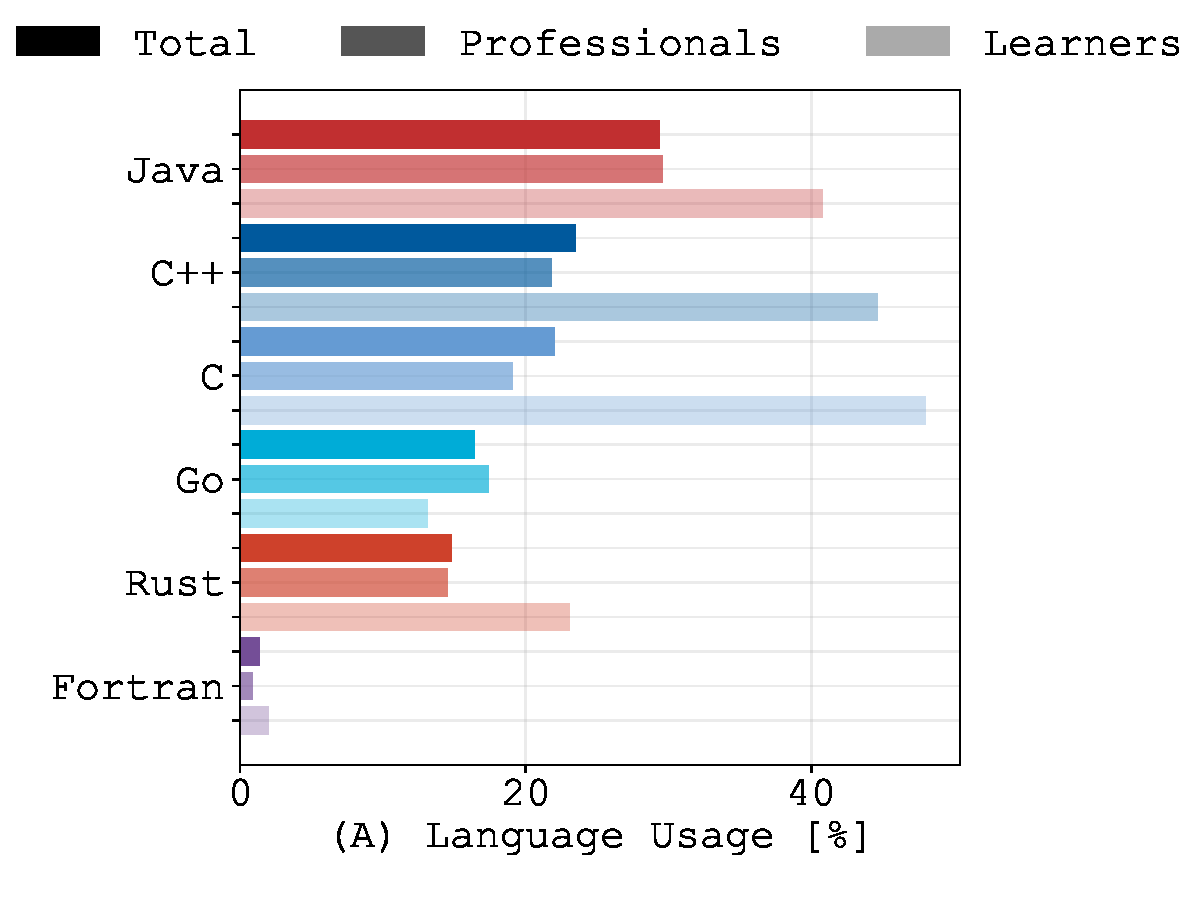
\includegraphics[width=0.5\textwidth]{figures/stackoverflow-popular-languages.pdf}%
    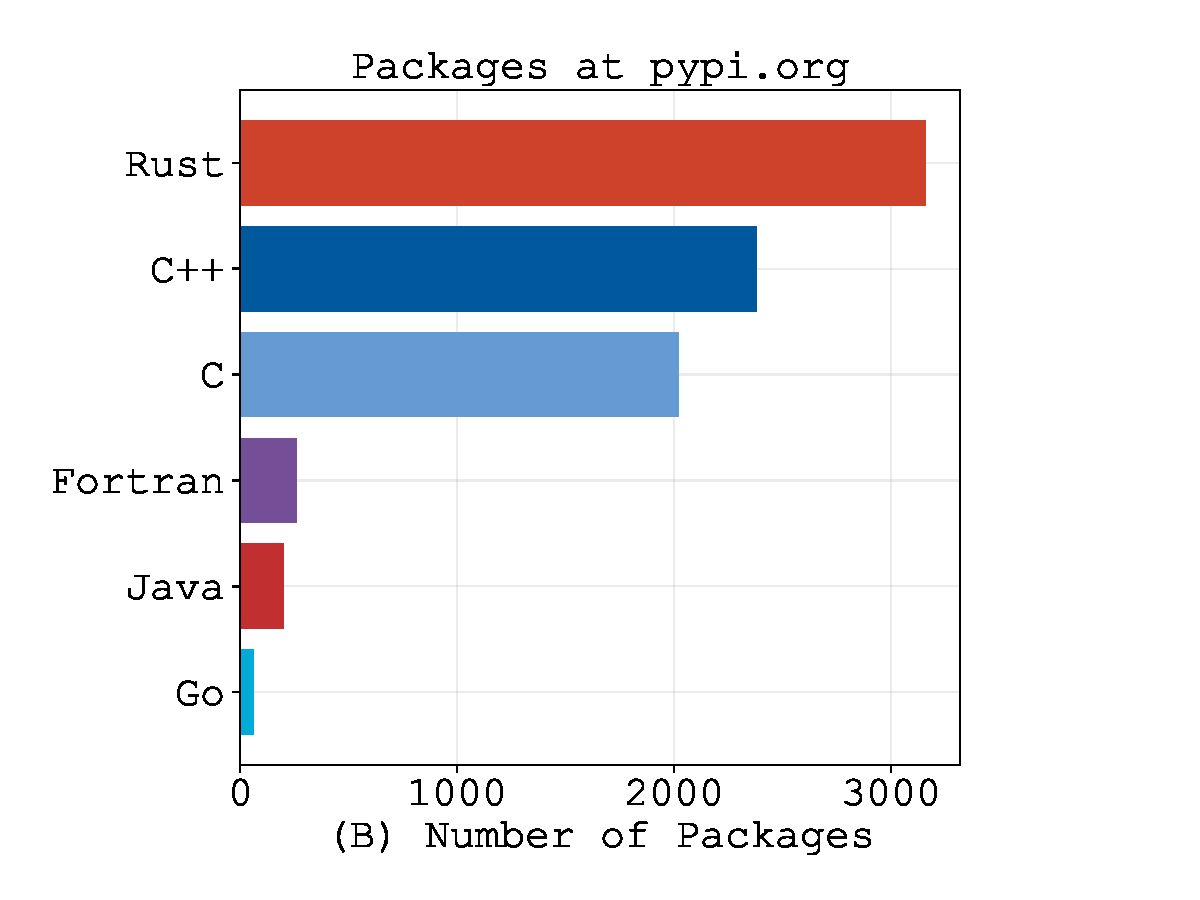
\includegraphics[width=0.5\textwidth]{figures/pypi-org-used-languages.pdf}
    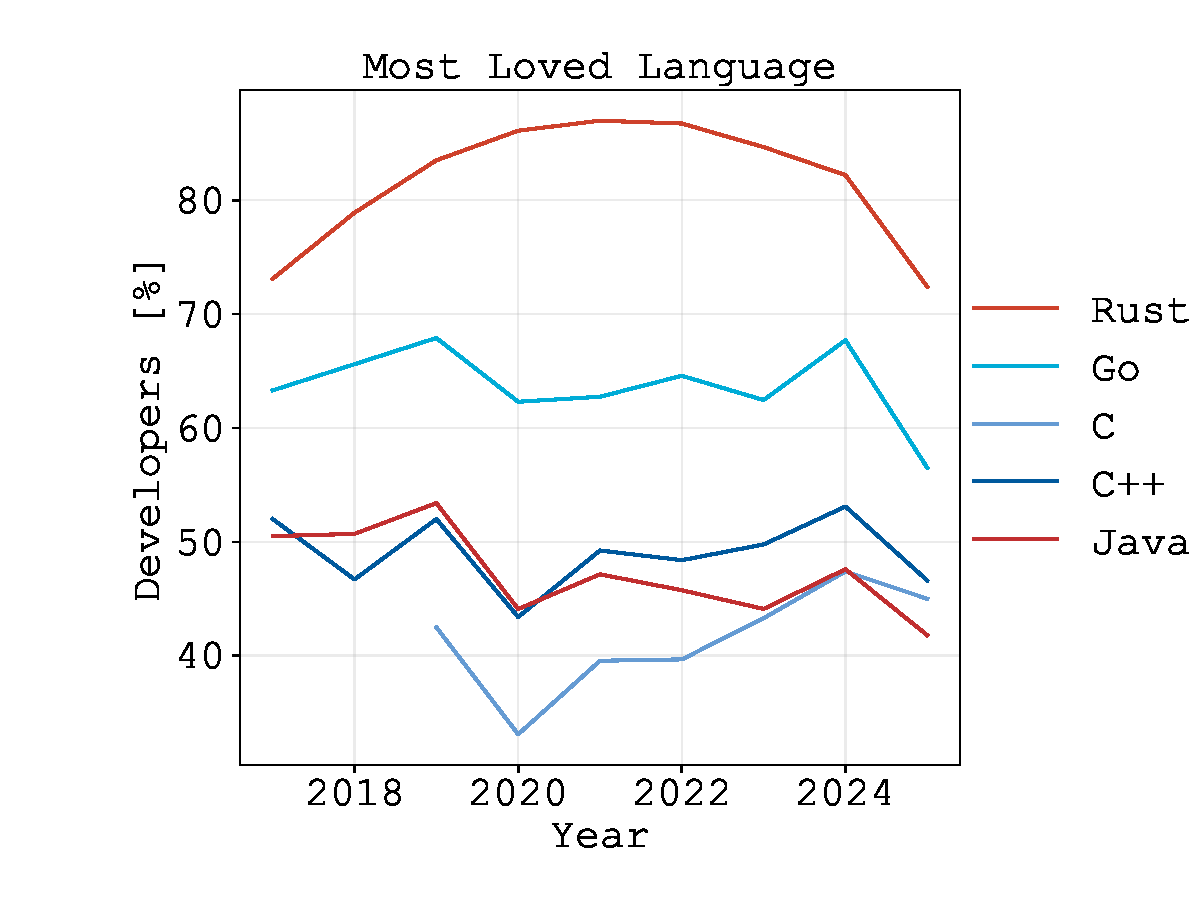
\includegraphics[width=0.5\textwidth]{figures/stackoverflow-loved-language.pdf}%
    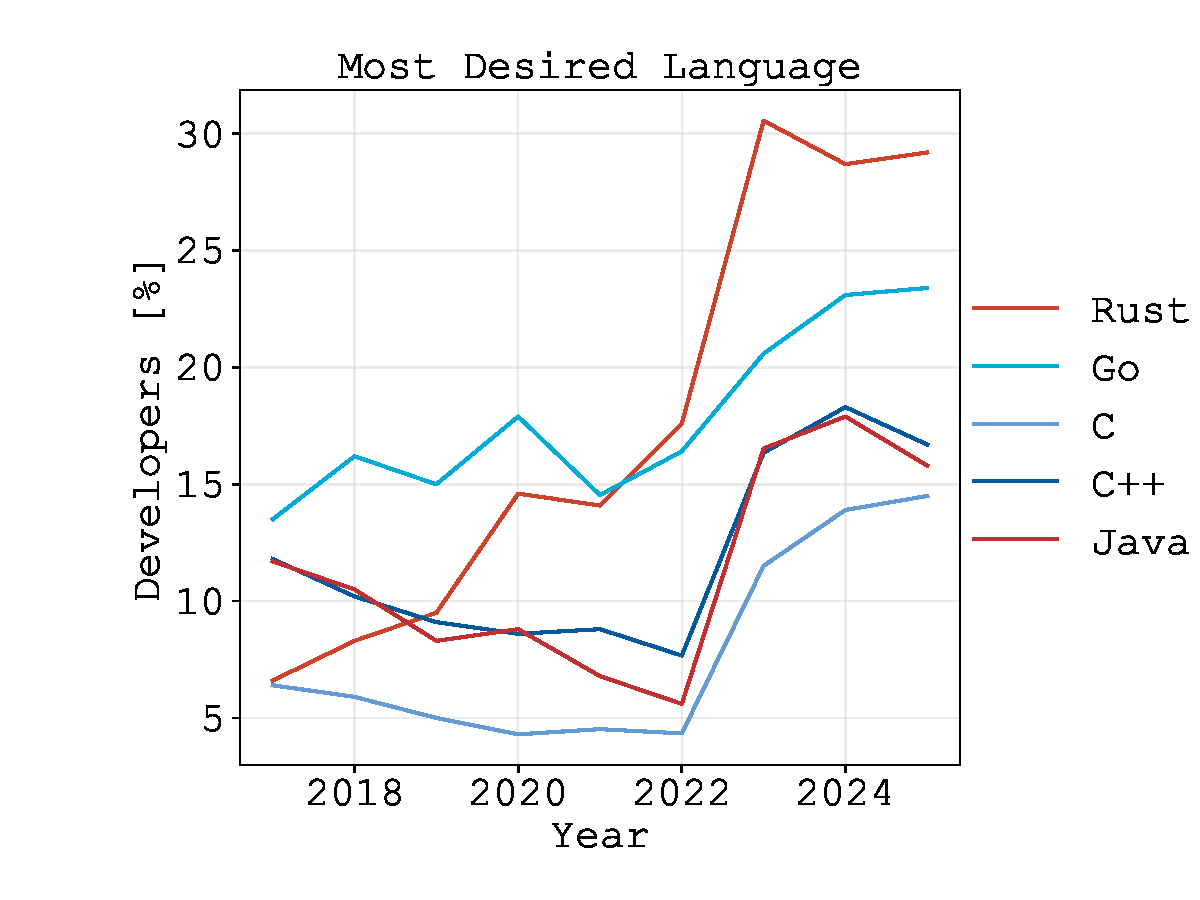
\includegraphics[width=0.5\textwidth]{figures/stackoverflow-desired-language.pdf}
    \caption{TODO}
\end{figure}

%###################################################################################################
\section{Ecosystem and Libraries}

\subsection{Foundational Components}
\subsubsection{Linear Algebra \& Arrays}
(nalgebra, ndarray) (dense, sparse matrices, solvers)

\subsubsection{Numerical Methods}
(floating point arithmetic, etc.)

\subsubsection{Statistics \& Probability}
(statrs, ndarray-stats, smartcore)

\subsubsection{Symbolic \& Algebraic Computing}
(num, rug, speciyl, symcc, enzyme)

\subsubsection{Datastructures}
(graphs, etc.)

\subsection{Computational Methods}
\subsubsection{Optimization}
\subsubsection{Differential Equations}
(ODEs, PDEs)

ODE solvers~\cite{Renevey2024}, Diffsol

\subsubsection{Physics Engines}
(Fluid Dynamics, Manybody)

salva (2D \& 3D)~\cite{Crozet2024}

Rapier (2D \& 3D)~\cite{Crozet2025}

\subsubsection{Numerical Integration \& Differentiation}
(quadrature, monte-carlo, symbolic diff, enzyme)

\subsubsection{(Probabilistic Algorithms)}

\subsection{High-Performance \& Scalable Computing}
\subsubsection{Parallel Computing}
(rayon, compare to openmp, MPI bindings)

\subsubsection{GPU \& Accelerators}
(rust-cuda, cudarc, wgpu~\cite{Fitzgerald2025}, opencl, mention SPIRV)

\subsubsection{Sparse \& Structured Computations}
(large databases)

\subsection{Creature Comforts}
\subsubsection{Debugging}
(Rust Errors as values, tracing, logging) ecosystem

\subsubsection{Storage}
(serde, json, xml, ron, ...)

\subsubsection{Bindings}
(pyo3, maturin, C, cxxbridge, cmake)

\subsection{Visualization}
\subsubsection{Plotting (2D)}
plotters, plotlib, gnuplot bindings

\subsubsection{3D Rendering}
vtk-rs

Meshing (honeycomb)

\subsubsection{Interactive}
(dioxus)

%###################################################################################################
\section{Applications}
\label{section:applications}

\subsection{Physics \& Engineering}
\subsection{Biology \& Chemistry}
\cite{Pleyer2024}, Computational Oncology~\cite{Köster2025}, Proteomics~\cite{Anechitoaie2024}
\subsection{Climate \& Earth Sciences}
\subsection{Economics \& Finance}
\subsection{Social Sciences}

%###################################################################################################
\section{Discussion}
\label{section:discussion}

%###################################################################################################
\section{Conclusion}
\label{section:conclusion}

\printbibliography

%###################################################################################################
\pagebreak
\newcounter{supplementSection}
\renewcommand{\thesubsection}{S\arabic{supplementSection}}
\newcommand{\supplement}[1]{%
    \stepcounter{supplementSection}%
    \subsection{#1}
}
\renewcommand{\thesection}{}

\section{Supplementary Material}
\supplement{List of all crates}

\paragraph{Scientific Computing in Rust monthly Newsletter}

approx-derive\\
A procedural macro that automatically implements approximate equality traits for
floating-point types and custom structs. It builds on the approx crate to make testing numerical
code easier. This helps ensure tolerance-based equality checks are consistent and less error-prone.

approxim\\
A library for approximation algorithms in numerical computing. It provides tools for
approximating functions, datasets, or computations efficiently. The focus is on balancing precision
with performance in scientific workflows.

bacon-sci\\
A scientific computing library built on Rust that provides a foundation for numerical
and algebraic operations. It aims to be a lightweight alternative to larger ecosystems. Its design
emphasizes safety, performance, and modularity.

cargo-upgrades\\
A Cargo subcommand for upgrading dependencies in a Rust project. It automates
version checking and updates Cargo.toml accordingly. This reduces the manual overhead of keeping
scientific projects up to date.

EGObox\\
A library for evolutionary game theory and agent-based modeling. It allows researchers to
explore strategies, equilibria, and dynamics in multi-agent systems. Designed with flexibility to
model diverse game-theoretic scenarios.

faer\\
A linear algebra library for Rust with focus on high-performance matrix operations. It
provides dense and sparse routines with attention to numerical stability. The crate aims to become
a foundation for scientific and machine-learning applications in Rust.

fact.rs\\
A crate for fast matrix factorizations and related linear algebra decompositions. It
provides algorithms like LU, QR, and eigenvalue methods. Its goal is to complement crates like faer
with specialized routines.

globalsearch\\
A Rust crate for global optimization and search algorithms. It supports solving
complex optimization problems where local minima are common. Useful in scientific simulations and
computational experiments.

indexing\_fmt\\
A utility crate for formatting indices and ranges in scientific computing contexts.
It makes working with slices and multi-dimensional arrays more ergonomic. This helps in debugging
and presenting results.

integraal\\
A symbolic and numerical integration library for Rust. It supports computing definite
and indefinite integrals for a variety of functions. Its goal is to provide a reliable integration
toolkit for researchers.

kifmm-rs\\
A Rust implementation of the kernel-independent fast multipole method (FMM). It
accelerates particle simulations and large-scale interactions in physics. The focus is on
high-performance computing and scalability.

ndgrid\\
A crate for generating multi-dimensional grids, similar to MATLAB’s ndgrid. It is
especially useful in scientific computing for parameter sweeps and simulations. Provides ergonomic
grid construction for Rust’s array ecosystem.

ndelement\\
A crate for manipulating individual elements in multi-dimensional arrays. It offers
convenient indexing and iteration across dimensions. Designed to complement libraries like ndarray.

ndarray\\
A core Rust crate for n-dimensional arrays, inspired by NumPy. It provides efficient
array structures, broadcasting, slicing, and linear algebra support. Widely used as a foundation
for many Rust scientific computing libraries.

ploc\\
A parallelized algorithm library for localization and clustering tasks. Focuses on scalable
implementations of clustering approaches. Intended for large datasets in scientific applications.

Polars\\
A fast DataFrame library for Rust, with APIs also available in Python. It provides
powerful data manipulation, joins, and group-by operations with performance close to Apache Arrow.
Designed for data science, analytics, and scientific workflows.

Quant-Iron\\
A crate for quantitative finance and scientific modeling. It implements financial
instruments, stochastic processes, and numerical solvers. Designed to bridge scientific computing
with financial applications.

paradis\\
A discrete dislocation dynamics simulator written in Rust. It is used in materials
science to model dislocation behavior under stress. The library emphasizes performance and
scalability for large simulations.

repgenerate\\
A tool for generating reproducible reports from computational experiments. It
integrates with Rust code to ensure scientific workflows can be repeated. Useful for open and
transparent research.

rsmpi\\
Rust bindings to the Message Passing Interface (MPI). It enables parallel computing across
distributed systems, a key component in HPC. Provides safe abstractions while maintaining low-level
control.

serde\\
A widely used Rust serialization and deserialization framework. It supports many formats
like JSON, YAML, and custom binary encodings. In scientific computing, it helps with data exchange
and configuration management.

sequenceprofiler\\
A bioinformatics library for profiling biological sequences. Provides tools for
analyzing DNA, RNA, or protein sequences. Aimed at high-performance sequence analysis in Rust.

zarrs\\
A Rust implementation of the Zarr data format for chunked, compressed N-dimensional arrays.
It allows efficient storage and manipulation of large scientific datasets. Especially useful in
machine learning and climate science.

\paragraph{JOSS}

fastatomstruct\\
A Rust library for high-performance analysis of atomic systems. It provides tools
for structural and dynamical computations, enabling simulations and data analysis in computational
chemistry and materials science. Optimized for speed, it can handle large datasets efficiently.

grepq\\
A Rust tool designed to process and filter FASTQ files efficiently. It matches sequences
against sets of regular expressions, making it useful for high-throughput sequencing data analysis.
Its focus is on speed and flexibility for genomic workflows.

pengWann\\
A library that computes chemical bonding descriptors using Wannier functions. It aids in
understanding electronic structure and bonding characteristics in materials. Suitable for quantum
chemistry and materials science applications.

wrenfold\\
A Rust library for symbolic computation and code generation tailored to robotics
applications. It allows automatic generation of control and kinematics code from symbolic
expressions. Supports efficient development of robotic algorithms.

kifmm-rs\\
A Rust framework implementing the kernel-independent fast multipole method (FMM). Used
to accelerate N-body computations in physics and engineering. Optimized for performance and
scalable to large simulations.

startinpy\\
A Python package for modeling and processing 2.5D terrains. Supports triangulated
meshes and geospatial analysis. Useful in geoscience, terrain analysis, and visualization.

Back to sequences\\
A tool for tracing the origins of k-mers in sequencing data. Helps analyze and
understand sequence composition and frequency. Useful for genomics and bioinformatics research.

sourmash v4\\
A bioinformatics toolkit for genome and metagenome analysis. Provides fast
comparison, search, and analysis of sequencing data. Supports scalable workflows with large
datasets.

extendr\\
A Rust library that facilitates seamless integration with the R programming language.
Allows calling Rust functions from R and vice versa. Focuses on performance and ease of use for
scientific computing.

Pywaterflood\\
A Python library for analyzing well connectivity in hydrogeology or petroleum
engineering. Uses capacitance-resistance modeling to simulate flow and connectivity. Supports
data-driven analysis for reservoir studies.

Gibbs Sea Water Oceanographic Toolbox\\
A Rust implementation of the TEOS-10 toolbox for
oceanographic computations. Provides tools for thermodynamic and salinity calculations in seawater.
Useful for oceanographers and climate researchers.

Raphtory\\
A toolkit for building and analyzing temporal graphs. Supports both Rust and Python
interfaces. Enables high-performance analytics on time-evolving network data.

HDT\\
A Rust library for working with HDT, a binary compression format for RDF data. Optimizes
storage and query of large knowledge graphs. Useful for semantic web and linked data applications.

egobox\\
A Rust toolbox for performing global optimization. Implements algorithms for efficiently
exploring high-dimensional spaces. Useful in engineering, machine learning, and simulation-based
optimization.

Fast k-medoids Clustering\\
A high-performance implementation of k-medoids clustering in Rust, with
Python bindings. Supports scalable clustering of large datasets. Ideal for machine learning and
data analysis tasks.

FEM\_2D\\
A Rust library for 2D finite element simulations. Supports hp-refinement for adaptive
mesh accuracy. Designed for engineering, physics, and numerical analysis applications.

retworkx\\
A Python graph library with Rust backend for performance. Supports graph creation,
traversal, and analysis. Useful in network science, bioinformatics, and algorithm development.

Rasusa\\
A bioinformatics tool for subsampling sequencing reads. Allows control of coverage in
genomic datasets. Helps optimize computational pipelines and reduce data size for analysis.

Sepia\\
A Rust tool for classifying sequencing reads by taxonomy. Provides high-performance
analysis for metagenomics studies. Helps researchers quickly categorize large datasets.

RustBCA\\
A Rust library implementing the binary collision approximation (BCA) for ion-material
simulations. Enables efficient modeling of particle interactions in materials. Used in physics and
materials research.

City2BA\\
A Rust package for generating synthetic bundle adjustment datasets. Useful in computer
vision and photogrammetry. Helps test and benchmark 3D reconstruction algorithms.

\paragraph{Scientific Computing in Rust 2025 talks}

Diffsol\\
A crate for solving differential equations.

Pixi\\
The missing companion to Cargo.

ploc\\
Efficient point location with ploc.

NPB-Rust\\
NAS parallel benchmarks in Rust.

cellular\_raza\\
Cellular agent-based modeling from a clean slate.

ninterp\\
Numerical interpolation in N-dimensions.

Arrow\\
Arrow, Rust, and cross-language data science tooling.

Juice\\
Juice your simulations: what science can learn from game development.

eVaiutilities\\
Research data management post eVai.

Honeycomb\\
Combinatorial maps implementation for meshing applications.

Stochastic\\
Stochastic calculus in Rust.

Exponential\\
Exponential time integration for stiff systems in Rust.

Rust\\
Rust for chip design algorithms and EDA software.

Using\\
Using Rust to mitigate breaking changes in scientific software.

The\\
The pleasure and pain of developing cross-platform CPU vector code in Rust.

Deimos\\
Open-source scientific data acquisition \& laboratory controls.

Rust\\
Rust is RAD and this is why.

Diffsol\\
A crate for solving differential equations.

Pixi\\
The missing companion to Cargo.

ploc\\
Efficient point location with ploc.

\paragraph{Scientific Computing in Rust 2024 talks}

AcoDyn\\
Fluid dynamics on the GPU powered by Rust.

rlst\\
The Rust Linear Solver toolbox is an in-development project for dense and sparse linear algebra routines in Rust.

Raphtory\\
Temporal graphs from Scala to Rust.

Bless\\
Transparently logging program outputs.

sophus-rs\\
A fast electromagnetics library with Rust and Python.

sophus-rs\\
A fast electromagnetics library with Rust and Python.

Rootfinders\\
Rootfinders for Rust.

Rstats\\
Multidimensional data analysis in Rust.

extendr\\
Frictionless bindings for R and Rust.

Rusting\\
Rusting RSRS.

Physics\\
Physics simulations in Bevy.

An\\
An embedded memory cache for persistent memory access.

Polars\\
Polars in the factory: when databases trump collections for modeling.

Perpetaul\\
Perpetaul: a hyperparameter-free gradient boosting machine.

Writing\\
Writing maths software in Rust after 20 years of C++: graph isomorphism and groups.

Productive\\
Productive and reliable constitutive modeling in Rust.

Efficient\\
Efficient 1-bit matrix approximations.

Developing\\
Developing Rust-based R packages using the Roxido framework.

Rusph\\
Rusph: a SPH astrophysical simulation code in the Rust programming language.

Back\\
Back to basics: rebuilding computational biomechanics crate by crate.

Cargo\\
Cargo +GPU build: An early outlook.

Writing\\
Writing a grid library for finite and boundary element methods.

\paragraph{Scientific Computing in Rust 2023 talks}

jiro\_nn\\
Low-friction high-detail Deep Learning framework in Rust

\url{https://chrisproject.org/}\\
ChRIS is an open-source platform for computational research and medicine.

struqture\\
Represent quantum mechanical operators, Hamiltonians and open quantum systems.
\url{https://quantumsimulations.de/}

salso, caviarpd, \& fangs\\
R extensions written in Rust

faer-rs\\
A linear algebra foundation for the Rust programming language.

Lamellar\\
A Rust-based asynchronous tasking and PGAS runtime for high-performance computing.

Sage\\
Enables fast proteomics searching and quantification at scale.

Bernstein–Bézier\\
Finite elements for RMM in Rust~\cite{Sky2024}

mwa\_hyperdrive\\
Calibration software for the Murchison Widefield Array (MWA) radio telescope.
\url{https://mwatelescope.github.io/mwa_hyperdrive/index.html}

alg\_tools\\
utility routines and tools for implementing iterative algorithms and (abstract) numerical computing in Rust~\cite{Valkonen2023}.
\url{https://tuomov.iki.fi/software/alg_tools/}

clarabel\\
Clarabel is an interior point numerical solver for convex optimization problems using a novel
homogeneous embedding~\cite{Clarabel_2024}.

fips\\
\cite{jeggle2023genericframeworkdataracefreemanyparticle}
\url{https://zenodo.org/records/6757615}

Roqoqo\\
A quantum computing toolkit in Rust.

Lace\\
Bayesian tabular data analysis for Rust (and Python).

Rudolph\\
Improving productivity of medical research with Rust CLI tools.

Rstats\\
Multidimensional data analysis in Rust.

extendr\\
Frictionless bindings for R and Rust.

Rusting\\
Rusting RSRS.

Physics\\
Physics simulations in Bevy.

An\\
An embedded memory cache for persistent memory access.

Polars\\
Polars in the factory: when databases trump collections for modeling.

Perpetaul\\
Perpetaul: a hyperparameter-free gradient boosting machine.

Writing\\
Writing maths software in Rust after 20 years of C++: graph isomorphism and groups.

Productive\\
Productive and reliable constitutive modeling in Rust.

Efficient\\
Efficient 1-bit matrix approximations.

Developing\\
Developing Rust-based R packages using the Roxido framework.

Rusph\\
Rusph: a SPH astrophysical simulation code in the Rust programming language.

Back\\
Back to basics: rebuilding computational biomechanics crate by crate.

Cargo\ \ Cargo +GPU build: An early outlook.

Writing\\
Writing a grid library for finite and boundary element methods.

\end{document}
